\section{Esempi di funtori nella pratica matematica}\label{sec_esempi_funtori}
\`E chiaro che non si può compilare una lista esaustiva di funtori importanti nella pratica matematica. Possiamo però concentrarci su alcuni funtori che è immediato costruire tra le categorie di §\ref{sec_esempi_cats}. In particolare, ed è uno dei motivi per cui \ref{def_funtore} è interessante, diverse operazioni che guardano una struttura come esempio di un'altra struttura si possono rendere precise mediante la nozione di funtore.
\begin{example}[Categorie discrete e codiscrete]\label{ex_fun_co_disc}\index{Categoria!--- discreta}\index{Categoria!--- codiscreta}\index{Funtore!--- categoria discreta}\index{Funtore!--- categoria codiscreta}
	Mandare un insieme \(A\) nella sua categoria discreta \(A^\delta\) di \ref{ex_cat_discreta} è un funtore \((\blank)^\delta : \ctSet \fun \ctCat\): ogni funzione \(f : A \to B\) induce un funtore, tautologico, \(f^\delta : A \to B\) che agisce come \(f\) sugli oggetti, ed è univocamente determinato dalla richiesta che \(f^\delta(\id_a) = \id_{fa}\), imposta da \ref{p_1}.

	Similmente, mandare un insieme \(A\) nella sua categoria codiscreta \(A^\chi\) è un funtore \(\ctSet \fun\ctCat\); qui è meno immediato che esista un funtore \(f^\chi : A^\chi\fun B^\chi\), ma usando la caratterizzazione di un funtore in \ref{def_alternativa_funtore} è sufficiente trovare una famiglia di funzioni
	\[\begin{tikzcd}
			f^\chi_{aa'} : \Hom{A^\chi}(a,a') \ar[r] & \Hom{B^\chi}(fa, fa')
		\end{tikzcd}\]
	e l'unica freccia \(u_{aa'} : a\to a'\) deve per forza essere mandata nell'unica freccia \(v_{fa,fa'} : fa \to fa'\) in \(B^\chi\).
\end{example}
\begin{example}\label{dom_e_cod}\index{Funtore!--- dominio}\index{Funtore!--- codominio}
	Se \(\ctC\) è una categoria e \(X\in\ctC_0\), esiste un funtore `dominio'
	\[\dmFun{d}{\ctC/X}{\ctC}\]
	che manda ogni oggetto \(f : A\to X\) di \(\ctC/X\) nel suo dominio \(A\).

	Similmente, esiste un funtore `codominio'
	\[\dmFun{c}{X/\ctC}{\ctC}\]
	che manda ogni oggetto \(f : X\to A\) nel suo codominio \(A\).
\end{example}
\begin{example}\index{Funtore!--- insieme delle parti}\label{ex_fun_parti}
	Ad ogni insieme possiamo associare il suo \emph{insieme delle parti}, l'insieme \(\pow X\) delle funzioni \(\chi : X \to \{0,1\}\); questo definisce l'azione sugli oggetti di un funtore \(\ctP : \ctSet\fun\ctSet\),	e in effetti, di due, uno covariante e uno controvariante:
	\begin{itemize}
		\item il \emph{funtore potenza covariante}, che manda una funzione \(f : X\to Y\) nella funzione
		      \[\dmFun{\ctP_* f}{\pow X}{\pow Y}\]
		      definita mandando \(\chi : X\to \{0,1\}\) nella funzione \[\ctP_* f(\chi)(y) := \begin{cases}
				      1 & \exists x . (y = fx) \land (\chi(x) = 1) \\
				      0 & \text{altrimenti}                        \\
			      \end{cases}\]
		\item il \emph{funtore potenza controvariante}, che manda una funzione \(f : X\to Y\) nella funzione
		      \[\dmFun{\ctP^* f}{\pow Y}{\pow X}\]
		      definita mandando \(\varpi : Y \to \{0,1\}\) nella funzione \(\ctP^* f(\varpi)(x) := \varpi(f(x))\).
	\end{itemize}
	In entrambi i casi, è semplice verificare che \(\ctP_* (g\cmp f) = \ctP_* g\cmp \ctP_* f\) (risp., \(\ctP^* (g\cmp f) = \ctP^* f\cmp \ctP^* g\)) e \(\ctP_*(\Id[X]) = \Id[\pow X] = \ctP^*(\Id[X])\); lo si faccia per esercizio.
\end{example}
\begin{definition}[Il funtore dei sottoggetti]\label{def_fun_sub}\index{Funtore!--- dei sottoggetti}
	Dato un insieme \(X\) consideriamo la classe di tutti i monomorfismi di codominio \(X\), cioè le funzioni iniettive \(A\mono X\); dati due monomorfismi \(m : A\mono X, n : B\mono X\), diciamo che \(m\le n\) se esiste una funzione (necessariamente un mono) \(h : A\to B\) tale che \(n\cmp h = m\); il triangolo commutativo
	% https://q.uiver.app/#q=WzAsMyxbMCwwLCJBIl0sWzAsMiwiQiJdLFsxLDEsIlgiXSxbMCwyLCJtIiwwLHsic3R5bGUiOnsidGFpbCI6eyJuYW1lIjoiaG9vayIsInNpZGUiOiJ0b3AifX19XSxbMSwyLCJuIiwyLHsic3R5bGUiOnsidGFpbCI6eyJuYW1lIjoiaG9vayIsInNpZGUiOiJ0b3AifX19XSxbMCwxLCJoIiwyLHsic3R5bGUiOnsidGFpbCI6eyJuYW1lIjoiaG9vayIsInNpZGUiOiJ0b3AifX19XV0=
	\[\begin{tikzcd}[row sep=2mm]
			A \\
			& X \\
			B
			\arrow["m", hook, from=1-1, to=2-2]
			\arrow["h"', hook, from=1-1, to=3-1]
			\arrow["n"', hook, from=3-1, to=2-2]
		\end{tikzcd}\]
	traduce il fatto che \(A\) è un sottoinsieme di \(X\), ma anche di un altro sottoinsieme \(B\), possibilmente più piccolo. Diciamo poi che \(m,n\) come sopra sono equivalenti, scritto \(m\simeq n\), se \(A\) e \(B\) sono isomorfi (per il teorema di Cantor-Schröder-Bernstein questo equivale a \(m\le n\) e \(n\le m\)).

	Il \emph{funtore dei sottoggetti}
	\[\dmFun{\Sub}{\ctSet^\op}{\ctSet}\]
	assegna a un insieme \(X\) l'insieme delle classi di equivalenza di mono \(\{m : A\mono X\}\) (che questo sia un insieme, segue dall'assioma dell'insieme potenza di ZF). L'azione sulle frecce si determina come segue: data una funzione \(f : X\to Y\), esiste una funzione
	\[\dmFun{\Sub(f)}{\Sub(Y)}{\Sub(X)}\]
	che manda \(U\subseteq Y\) nel sottoinsieme \(\ctP^*(f)[U]\) come definito sopra.

	La presenza di un isomorfismo naturale tra il funtore dei sottoggetti \(\Sub\) e \(\ctP^*\), come funtori di tipo \(\ctSet^\op\fun\ctSet\), si basa sull'esistenza di una famiglia di biiezioni \(\chi_X : \ctP(X) = \pow X \cong \{U\subseteq X\}\)
\end{definition}
\begin{example}[Monoidi come categorie]\label{funtore_mon_to_cat}\index{Funtore!--- categoria associata a monoide}
	La corrispondenza che assegna a un monoide \((M,\cdot,1)\) la categoria con un solo oggetto \(\susp(M,\cdot,1)\) come in \ref{mon_sonocat} è la parte sugli oggetti di un funtore
	\[\dmFun{\susp}{\ctMon}{\ctCat}\]
	tra le categorie di \ref{ex_cat_monoidi} e di \ref{ex_cat_cat}; abbiamo in effetti già dimostrato in \ref{exa_funtori_da_gruppi} che i funtori tra categorie della forma \(\susp M\) sono tutti e soli gli omomorfismi di monoidi (e la composizione di omomorfismi \(M\to N\to R\) e di funtori \(\susp M \fun\susp N \fun\susp R\) coincidono), quindi la sottocategoria di \(\ctCat\) identificata come l'immagine di \(\susp\) è piena, e si identifica alla categoria dei monoidi. (Questa ultima osservazione sarà chiara quando avremo introdotto la nozione di \emph{funtore pienamente fedele} in \ref{fun_pienfed}.)
\end{example}
\begin{remark}[Ordini come categorie]\label{ord_come_cat}\index{Preordine}\index{Preordine!---i come categorie}
	In maniera analoga la corrispondenza che assegna a un insieme ordinato \((P,\le)\) la categoria definita in \ref{ord_sonocat} è la parte sugli oggetti di un funtore
	\[\dmFun{t}{\ctPos}{\ctCat.}\]
	Grazie a \ref{exa_monotone_funtori}, i funtori tra categorie della forma \(t(P,\le)\) sono tutte e sole le funzioni monotòne nel senso di \ref{ex_cat_ordini}.

	\`E usuale non denotare in alcun modo particolare questo funtore, cosicché `considerare la categoria \((P,\le)\)' ha come unico significato possibile considerare la categoria \(t(P,\le)\) i cui oggetti sono \(p\in P\) e dove c'è esattamente una freccia \(p\to p'\) se e solo se \(p\le p'\).
\end{remark}
\index{Funtore!--- pieno}
\index{Funtore!--- fedele}
\index{Funtore!--- pienamente fedele}
\begin{example}[Le componenti connesse di un (multidi)grafo]\index{Funtore!--- componenti connesse di un grafo}\index{aaa_pi0@\(\pi_0\)|see {componenti connesse}}\index{Componenti connesse!--- di un grafo}\label{ex_fun_cpt_conn}
	Se \(\ctG=(E,V)\) è un multidigrafo come in \ref{ex_cat_grafi}, possiamo costruire l'insieme delle sue \emph{componenti connesse} considerando la relazione \(x\asymp y\) sull'insieme dei suoi vertici, definita da \(x\asymp y\) se \(x=y\), o esiste un lato \(e : x \to y\), o esiste un lato \(e' : y\to x\). Due vertici \(x,y\in V\) appartengono alla stessa componente connessa se esiste una successione finita di vertici \(\tup vn,\) tale che
	\[x \asymp v_1 \asymp v_2 \asymp\dots\asymp v_n\asymp y.\]
	(Si tratta in poche parole della chiusura transitiva \(\asymp^*\) di \(\asymp\), che quindi diventa una relazione di equivalenza su \(V\).)

	Definiamo \(\pi_0\ctG\) come l'insieme quoziente \(V/_{\asymp^*}\) delle componenti connesse di \(\ctG\). Questa assegnazione è la funzione sugli oggetti di un funtore
	\[\dmFun{\pi_0}{\ctdGph}{\ctSet}\]
	che su un omomorfismo di multidigrafi \(f : \ctG \to\ctH\) è definita mandando la componente connessa di \(v\in V_\ctG\) nella componente connessa di \(f_V(v)\in V_\ctH\) (è immediato verificare dal fatto che \(f_E(e : x\to y)=f_Ee : f_Vx\to f_Vy\) che questa è una buona definizione, cioè che \(f_V\) scende al quoziente).
\end{example}
\begin{example}[La categoria libera associata a un grafo]\index{Funtore!--- categoria libera}
	Se \(\ctG\) è un multidigrafo come in \ref{ex_cat_grafi}, la costruzione della categoria libera \(\bfF\ctG\) di \ref{ex_cat_libera} definisce la funzione sugli oggetti di un funtore
	\[\dmFun F\ctdGph\ctCat\]
	Un omomorfismo di grafi \((f_E,f_V) : \ctG \to \ctH\) infatti è il dato sufficiente per definire un funtore \(F(f_E,f_V) : \bfF\ctG \fun F\ctH\) sugli oggetti (con \(f_V\)) e sui morfismi generatori (con \(f_E\)), mandando la successione di lati contigui \([\tup en;]\) in \(\bfF\ctG\) in \([\tup {{f_E}e}n;]\) in \(F\ctH\) (se \(n=0\) questo significa che \(F(f_E,f_V)\emptyList = \emptyList\)).
\end{example}
\begin{example}[Realizzare \(\ctMat\) in \(\ctVect\)]\index{Funtore!--- matrici reali}
	La categoria delle matrici \(\ctMat\) è stata definita in \ref{ex_cat_matrici}; la categoria \(\ctVect\) è stata definita tra gli esempi di \ref{varie_categorie_nella_pratica}. Abbiamo già osservato che \(\ctMat\) si ottiene da \(\ctVect\) scegliendo un solo oggetto per ogni dimensione, e questo definisce un funtore ovvio \(\ctMat \to \ctVect\) (mandando \(n\) in \(\bbF^n\) e una matrice \(A\) nell'applicazione lineare che agisce come \(A\) nella base canonica). Esiste anche un funtore nella direzione opposta,
	\[\dmFun{Q}{\ctVect}{\ctMat}\]
	che assegna a uno spazio vettoriale \(V\) la sua dimensione (rispetto a una base scelta), e ad una mappa \(\bbF\)-lineare \(f : V\to W\) tra spazi vettoriali la matrice di \(f\) nelle basi scelte su \(V\) e \(W\).

	Più precisamente, la base \(b(V)\) è stata scelta per determinare un isomorfismo \(\theta_V : V \to \bbF^n\) (se \(n=\dim_\bbF V)\), e il quadrato di applicazioni lineari
	% https://q.uiver.app/#q=WzAsNCxbMCwwLCJWIl0sWzAsMSwiVyJdLFsxLDAsIlxcYmJGXm4iXSxbMSwxLCJcXGJiRl5tIl0sWzAsMSwiZiIsMl0sWzAsMiwiXFx0aGV0YV9WIl0sWzEsMywiXFx0aGV0YV9XIiwyXSxbMiwzLCJRZiJdXQ==
	\[\begin{tikzcd}[cramped]
			V & {\bbF^n} \\
			W & {\bbF^m}
			\arrow["{\theta_V}", from=1-1, to=1-2]
			\arrow["f"', from=1-1, to=2-1]
			\arrow["Qf", from=1-2, to=2-2]
			\arrow["{\theta_W}"', from=2-1, to=2-2]
		\end{tikzcd}\]
	è commutativo. Chi legge riconoscerà nella dimostrazione, lasciata per esercizio, delle proprietà \ref{f_1}, \ref{f_2} alcuni fatti fondamentali insegnati in algebra lineare.
\end{example}
\begin{example}[Successioni simmetriche, specie combinatorie]\index{Funtore!--- specie combinatoria}\index{Specie combinatoria}\index{Successione simmetrica|see {Specie combinatoria}}
	Si ricordi la definizione della categoria \(\cate{Bij}\) in \ref{ex_cat_gruppoide_naturali}; un funtore
	\[\dmFun{f}{\cate{Bij}}{\ctSet}\]
	consta dei seguenti dati:
	\begin{itemize}
		\item una collezione di insiemi \(f(n)=X_n\) indicizzata dai numeri naturali \(n\ge 1\);
		\item una rappresentazione \(S_n \times X_n\to X_n\), ossia un'azione (sinistra) del gruppo simmetrico \(S_n\) degli automorfismi dell'insieme \(\{\iter n\}\).
	\end{itemize}
	Il funtore \(f\) si dice una \emph{specie combinatoria} e la famiglia \(f(n)=X_n\) è una \emph{successione simmetrica}. Questo tipo di funtori, molto ricchi di struttura e di proprietà interessanti, trovano applicazioni in combinatoria enumerativa \cite{bergeron1998combinatorial}, teoria delle rappresentazioni \cite{aguiar2010monoidal}, geometria e topologia \cite{fresse-operads} (quando invece che insiemi gli \(X_n\) sono spazi vettoriali), logica e informatica teorica \cite{Gambino2017,Hasegawa2002}. Denotando con \(\# S\) la cardinalità di un insieme, ad ogni specie combinatoria \(f : \cate{Bij} \fun\ctSet\) tale che ogni \(f(n)\) sia finito possiamo associare la serie formale \(F(t)\in\mathbb{N}\llbracket t\rrbracket\) definita come \(F(t) \defeq \sum_{n\ge 1} \frac{\# X_n}{n!}t^n\). Questa si chiama la \emph{funzione generatrice} della specie combinatoria \(F\), e le sue proprietà algebriche o analitiche (qualora \(F(t)\) converga) sono in corrispondenza diretta con le proprietà del funtore \(f\).
\end{example}
\begin{example}[Moduli sinistri; moduli destri; bimoduli]\index{Moduli su un anello!--- come funtori}\index{Modulo}
	Se \(\ctAb\) è la categoria dei gruppi abeliani e loro omomorfismi, ed \((R,+,\cdot,0,1)\) è un anello unitario, una rappresentazione del monoide \((R,\cdot,1)\) in \(\ctAb\), ossia un funtore
	\[\dmFun{M}{\susp(R,\cdot,1)}{\ctAb}\]
	consiste di un gruppo abeliano \(M\) su cui è definita un'azione \(a\) del monoide \((R,\cdot,1)\) mediante mappe bilineari. L'azione \(a : R\times M\to M\) soddisfa cioè le proprietà
	\begin{itemize}
		\item \(a(1,m)=m\) per ogni \(m\in M\);
		\item \(a(s\cdot r,m)=a(s,a(r,m))\) per ogni \(r,s\in R\), \(m\in M\);
		\item \(a(r+s,m) = a(r,m) + a(s,m)\) per ogni \(r,s\in R\), \(m\in M\);
		\item \(a(r,m+n) = a(r,m) + a(r,n)\) per ogni \(r\in R\), \(m,n\in M\).
	\end{itemize}
	Denotando \(a(r,m)\) con un simbolo infisso \(r.m\), questi assiomi sono esattamente quelli che caratterizzano \(M\) come un \emph{\(R\)-modulo (sinistro)}.

	Similmente, un modulo destro è un funtore \emph{controvariante} \(R\fun\ctAb\), cioè un funtore \(R^\op\fun\ctAb\) dove \(R^\op\) è l'\emph{anello opposto} (cf. \ref{mon_opposti_cat_opposte}) dotato della moltiplicazione \(x\cdot^\op y \defeq y\cdot x\), e un \(R,S\)-\emph{bimodulo} è un funtore
	\[\dmFun{{}_RM_S}{S^\op\times R}{\ctAb.}\]
\end{example}
\begin{example}[Spazio delle orbite di un \(G\)-insieme]\index{Funtore!--- orbite di un \(G\)-insieme}\label{ex_fun_orbite}
	Ogni volta che sia data una rappresentazione di un gruppo \(G\) come in \ref{exa_azioni_funtori} (cioè un \(G\)-insieme come in \ref{ex_cat_g_insiemi}) possiamo considerare lo \emph{spazio delle orbite} \(X/G\) definito come l'insieme delle classi di equivalenza della forma
	\[[x]_G \defeq \{g\cdot x\mid g\in G\}\]
	(ciascuno dei \([x]_G\) si chiama l'\emph{orbita} di \(x\) rispetto all'azione di \(G\)).

	Mostriamo che esiste un funtore
	\[\dmFun{-/G}{G\emdash\ctSet}{\ctSet}\]
	che manda il \(G\)-insieme \(X\) nell'insieme \(X/G\). Affinché questo sia vero, una funzione equivariante \(f : X\to Y\) deve indurre una funzione ben definita tra gli spazi delle orbite \(X/G\) e \(Y/G\), in modo che gli assiomi \ref{p_1} e \ref{p_2} siano soddisfatti. \`E facile verificare che \(f/G : X/G \to Y/G : [x]_G\mapsto [f(x)]_G\) ha tutte queste proprietà. (In particolare, se chiamiamo \(\pi_X : X\to X/G\) la funzione \(x\mapsto [x]_G\) che manda ogni elemento nella sua orbita, \(f/G\) è l'unica funzione tale che \(f/G(\pi_X(x)) = \pi_Y(f(x))\).)
\end{example}
\begin{example}\index{Funtore!--- gruppo delle unità}
	Assegnare a un anello unitario \((R,+,0\cdot,1)\) il gruppo \((R^\times,\cdot,1)\) dei suoi elementi invertibili è un funtore
	\[\dmFun{(\blank)^\times}\ctRing{\ctGrp.}\]
	Infatti ogni omomorfismo di anelli \(f : R\to S\) induce un omomorfismo di gruppi \(f^\times : R^\times \to S^\times\), dato che se \(u\in R\) è invertibile, tale è anche \(f(u)\) (e \(f(u)^{-1}=f(u^{-1})\)).
\end{example}
\begin{example}\index{Funtore!--- di abelianizzazione}
	Dato un gruppo \(G\), il sottogruppo \([G,G]\) generato dai commutatori \([x,y] \defeq xyx^{-1}y^{-1}\) è il sottogruppo normale più piccolo tale che \(G/N\) sia abeliano; il quoziente \(G^\aa \defeq G/[G,G]\) si chiama \emph{abelianizzato} di \(G\) e l'assegnazione \(G\mapsto G^\aa\) definisce un funtore
	\[\dmFun{(\blank)^\aa}\ctGrp\ctAb\]
	di abelianizzazione. Un omomorfismo di gruppi \(f : G \to H\) infatti scende al quoziente ad un omomorfismo \(f^\aa : G^\aa \to H^\aa\) tale che
	\[
		\begin{tikzcd}
			G\ar[r, "f"]\ar[d, "\pi"'] & H \ar[d, "\pi"]\\
			G^\aa \ar[r, "f^\aa"']& H^\aa
		\end{tikzcd}
	\]
	sia commutativo (questo è evidente, dato che \(f[x,y]=[fx,fy]\)). L'omomorfismo \(f^\aa\) è l'unico con questa proprietà, e ciò mostra che \((g\cmp f)^\aa = g^\aa\cmp f^\aa\) e \((\id_G)^\aa=\id_{G^\aa}\).
\end{example}
\begin{example}\index{Funtore!--- campo dei quozienti}
	Se \(R\) è un dominio di integrità, il suo \emph{campo dei quozienti} \(Q(R)\) è l'anello definito come segue:
	\begin{itemize}
		\item i suoi elementi sono classi di equivalenza \(\frac pq\) di coppie \((p,q) \in R\times R\) dove \(q\ne 0\) rispetto alla relazione che identifica \((p,q), (p',q')\) quando \(pq'=qp'\);
		\item la somma e il prodotto sono definiti da
		      \[\frac pq + \frac st = \frac{pt+qs}{qt} \qquad\qquad \frac pq\cdot\frac st = \frac{ps}{qt}\]
	\end{itemize}
	Con queste scelte, \(Q(R)\) diventa un campo (cioè, ogni elemento diverso dalla classe di equivalenza di \((0,1)\) è invertibile).

	La corrispondenza \(R\mapsto Q(R)\) è la funzione sugli oggetti di un funtore
	\[\dmFun Q\ctDInt\ctFld\]
	(il dominio è la categoria degli anelli integri, il codominio è la sottocategoria -piena- di \(\ctcRing\) i cui oggetti sono i campi). Infatti, ogni omomorfismo di anelli \(f : R \to S\) che siano domini di integrità induce un omomorfismo di anelli \(Q(f) : Q(R) \to Q(S)\) definito da \(f(\frac pq) = \frac{fp}{fq}\).
\end{example}
\begin{example}[I gruppi lineari come funtori]\label{ex_fun_GLn}\index{Funtore!--- gruppo generale lineare}\index{GL|see {Gruppo generale lineare}}\index{Gruppo generale lineare}
	Se \(n\ge 1\) è un numero intero, mandare un anello commutativo \(R\) nel gruppo delle matrici invertibili \(n\times n\) a coefficienti in \(R\) è la funzione sugli oggetti di un funtore
	\[\dmFun{\GL_n}\ctcRing\ctGrp\]
	Per vederlo, basta definire un omomorfismo di gruppi \(\GL_n(f) : \GL_n(R)\to \GL_n(S)\) dato un omomorfismo di anelli \(f : R\to S\); ragioniamo nel caso \(n=2\) per comodità, e il caso generale è completamente analogo: la corrispondenza
	\[\GL_2(f) : A=\left(\begin{smallmatrix}
				a	&	b \\
				c	&	d
			\end{smallmatrix}\right)
		\mapsto
		\left(\begin{smallmatrix}
				fa	&	fb \\
				fc	&	fd
			\end{smallmatrix}\right)
	\]
	è tale che \(\det(\GL(f)A)=\det\left(\begin{smallmatrix}		fa	&	fb \\		fc	&	fd	\end{smallmatrix}\right) = f(\det A)\), cosicché \(\GL_2(f)\) è ben definita verso \(\GL_2(S)\); evidentemente ciascun \(\GL_2(f)\) è un omomorfismo di gruppi, e \(f\mapsto\GL_2(g\cmp f) = \GL_2(g)\cmp\GL_2(f)\), e \(\GL_2(\id_R) = \id_{\GL_2(R)}\).
\end{example}
\begin{example}\label{ker_e_coker}\index{Funtore!--- nucleo e conucleo}\index{ker|see {nucleo}}\index{coker|see {conucleo}}
	Data una applicazione lineare \(f : V\to W\) tra \(k\)-spazi vettoriali, il suo \emph{nucleo} consiste del sottospazio \(\ker f\le V\) di tutti i vettori \(v\in V\) tali che \(f(v)=0\). Questa assegnazione è un funtore
	\[\dmFun{\ker}{\ctVect^\to}\ctVect\]
	dove \(\ctVect^\to\) è la categoria delle frecce di \ref{def_cat_frecce}. Infatti, a ogni quadrato commutativo
	\[\begin{tikzcd}
			V \ar[r, "f"]\ar[d, "p"']& W\ar[d, "q"] \\
			V' \ar[r, "{f'}"'] & W'
		\end{tikzcd}\]
	corrisponde una mappa lineare \(\ker f \to \ker f'\) (la restrizione di \(p\) a \(\ker f\), dato che se \(fv=0\) anche \(f'(pv)=q(fv)=q(0)=0\)).

	Dualmente, il \emph{conucleo} di \(f : V\to W\) è lo spazio vettoriale quoziente \(W/fV\), e l'assegnazione \(f\mapsto \coker f\) è un funtore
	\[\dmFun{\coker}{\ctVect^\to}\ctVect\]
	perché un quadrato commutativo come sopra implica che \(q\) scende al quoziente in modo che composizione e identità siano rispettate: se \(F = fV\) è l'immagine di \(f\) in \(W\) ed \(F'\) quella di \(f'\) in \(W'\), la classe laterale \(w + F\) viene mandata in \(qw+F'\); questa è una buona definizione, perché \(q(fv) \in F'\) per ogni \(v\in V\).
\end{example}
\begin{example}\index{Funtore!--- di compattificazione}
	Se \((X,\tau)\) è uno spazio topologico come in \ref{ex_cat_top}, la sua \emph{compattificazione ad un punto}, o compattificazione di Alexandroff, è lo spazio topologico \((X_\infty,\bar\tau)\) dove \(X_\infty \defeq X + \{\infty\}\) è l'unione disgiunta di \(X\) e di un `punto all'infinito' \(\infty\), e \(\bar\tau\) è la topologia che contiene tutti gli aperti di \(\tau\) ma anche gli insiemi della forma \(K^c \cup \{\infty\}\), dove \(K\Subset X\) è un sottoinsieme chiuso e compatto di \(X\) e \(K^c = X\smallsetminus K\) è il suo complementare. Si osservi che
	\begin{itemize}
		\item \(X_\infty\) è compatto e contiene \(X\) come un sottospazio denso;
		\item \(X\mapsto X_\infty\) è un funtore
		      \[\dmFun{(\blank)_\infty}\ctTop\ctTop\]
		      (la cui immagine però è la sottocategoria degli spazi compatti), che induce, per ogni mappa propria \(f : X\to Y\), una mappa propria tra le loro compattificazioni
		      \[\begin{tikzcd}
				      f_\infty : X_\infty \ar[r] & Y_\infty
			      \end{tikzcd}\]
		      che manda \(x\mapsto fx\) e \(\infty_X\) in \(\infty_Y\). La continuità sugli aperti della topologia di \(Y\) è ovvia, e va verificata solo sugli aperti di \(Y_\infty\) della forma \(V=K^c\cup\{\infty_Y\}\) con \(K\) compatto e chiuso in \(Y\); del resto, ora, \(f^{-1}V = (f^{-1}K)^c \cup \{\infty_X\}\) che è un intorno aperto di \(\infty_X\) (essendo \(f\) propria, \(f^{-1}K\) è compatto).
	\end{itemize}
\end{example}
\begin{example}\label{fun_ex_omoto_omolo}\index{Funtore!--- omotopia}\index{Funtore!--- omologia}
	Ad ogni spazio topologico puntato \((X,x_0)\) si può associare l'insieme delle classi di omotopia di mappe \((S^1, \copmap[r] 10)\to (X, x_0)\) che preservano il punto base; tale insieme è un gruppo, e dato che la relazione di omotopia è una \emph{congruenza} rispetto alla composizione (ossia che, se \(f\cong g\) allora ogni volta che ciò ha senso si ha \(h\cmp f\cmp k\cong h\cmp g\cmp k\)), è anche un funtore
	\[\dmFun{\pi_1}\ctTop\ctGrp\]
	e in effetti, dato che mappe omotope \(f\cong g : X\to Y\) inducono lo stesso omomorfismo \(f_* = g_* : \pi_1(X,x_0) \to \pi_1(Y,y_0)\), un funtore
	\[\dmFun{\pi_1}\ctHoTop\ctGrp\]
	dove \(\ctHoTop\) è la categoria dell'omotopia di \ref{ex_cat_hotop}.

	Similmente (per chi avesse già familiarità con queste definizioni), i gruppi di omotopia superiore \(\pi_n(X,x_0) \defeq [(S^n,\copmap[r] 1{\mathbf{0}}), (X,x_0)]\) definiscono dei funtori\footnote{Pensando \(S^n\subseteq\bbR^{n+1}\), come il sottospazio \(\{x\in\bbR^{n+1}\mid \|x\|^2=1\}\) il suo punto base è \(\copmap[r]1{\mathbf 0}=(1,0,\dots,0)\).}
	\[\dmFun{\pi_n}\ctHoTop\ctAb\]
	e altrettanto fanno i funtori di omologia (a coefficienti interi)
	\[\dmFun{H_n(-,\bbZ)}\ctHoTop\ctAb\]
	per \(n\ge 0\), e di coomologia (a coefficienti interi)
	\[\dmFun{H^n(-,\bbZ)}{\ctHoTop^\op}{\ctAb.}\]
\end{example}
\begin{definition}\label{def_insieme_simpliciale}
	\index{Insieme!--- simpliciale}
	Un \emph{insieme simpliciale} consta di un funtore \(X_* : \bsDelta^\op\fun\ctSet\), dove \(\bsDelta\) è la categoria dei simplessi di \ref{rmk_delta_e_deltaPlus}.

	Quando la definizione di insieme simpliciale viene data esplicitamente, essa consiste del dato di:
	\begin{itemize}
		\item Una famiglia di insiemi \(X_0,X_1,\dots,X_n,\dots\); gli elementi di \(X_n\) sono detti	\emph{\(n\)-simplessi} di \(X_*\);
		\item Una famiglia di funzioni \(d_i^n : X_n\to X_{n-1}\), dette \emph{facce}, per \(0\leq i\leq n\); la faccia \(d_i^n(t)\) di un \(n\)-simplesso \(t\) è detta \emph{\(i\)-esima faccia} di \(t\);
		\item Una famiglia di funzioni \(s_i^n : X_n\to X_{n+1}\), dette \emph{degenerazioni}, per \(0\leq i\leq n\).
	\end{itemize}
	Questi dati sono soggetti (per funtorialità) alle \emph{identità simpliciali}: se \(X(\delta_n^i) := d_i\) e \(X(\sigma_n^i) := s_i\), allora
	\begin{gather}
		d_i\cmp d_j = d_{j-1}\cmp d_i, \quad i < j\label{idsim_1}\\
		s_i \cmp s_j = s_{j+1} \cmp s_i, \quad i \leq j\label{idsim_2}\\
		d_i\cmp s_j =
		\begin{cases}
			s_{j-1}\cmp d_i, & i < j      \\
			\id,             & i = j, j+1 \\
			s_j\cmp d_{i-1}, & i > j+1.
		\end{cases}\label{idsim_3}
	\end{gather}
	\`E proprio la funtorialità di \(X\), e la possibilità di decomporre ogni freccia di \(\bsDelta\) mediante facce e degenerazioni che ora implica che le identità simpliciali siano una condizione necessaria e sufficiente per definire un funtore \(X : \bsDelta^\op\fun\ctSet\).
\end{definition}
\begin{hRemark}[Cos'è esattamente un \(n\)-simplesso?]{tech}\index{Simplesso}\index{Insieme simpliciale}
	Gli elementi degli insiemi \(X_0, X_1\) in un insieme simpliciale \(X\) si possono pensare come lati di un grafo diretto con la coppia di funzioni \((d_1,d_0) : X_1 \to X_0\times X_0\) a fare da mappe di dominio e codominio (in \emph{questo} ordine: \(d_i = X(\delta^1_i)\) restringe \(X\) al vertice che \emph{non} contiene \(i\)), e gli elementi di \(X_2\) si possono rappresentare come dei `triangoli diretti': se \(t\in X_2\), possiamo considerare le sue facce \(d_i = X(\delta^2_i)\), ciascuna definita restringendo \(X\) al lato che \emph{non} contiene l'indice \(i\); le tre identità simpliciali quando \(n=1\) sono quindi
	\[
		d_0\cmp d_1 = d_0\cmp d_0,\quad
		d_0\cmp d_2 = d_1\cmp d_0,\quad
		d_1\cmp d_2 = d_1\cmp d_1
	\]
	cosa che implica che i lati di \(t\) si `incollino' a formare un triangolo del tipo
	\[\xymatrix{
			{\begin{smallmatrix}
						d_1d_1t \\
						d_1d_2t
					\end{smallmatrix}}
			\ar[rr]^{d_1t}\ar[dr]_{d_2t}&& {\begin{smallmatrix}
						d_0d_1t \\
						d_0d_0t
					\end{smallmatrix}}
			\\
			&{\begin{smallmatrix}
						d_0d_2t \\
						d_1d_0t
					\end{smallmatrix}}\ar[ur]_{d_0t}\ar@{}[u]|-t &
		}\]
	Ovviamente, è assai sconveniente denotare i vertici di un 2-simplesso a questa maniera; perciò si nominano \(a = d_1d_1t, c = d_0d_1t, b = d_0d_2t\) e si disegna più semplicemente un triangolo fatto da \(a \xto{d_2t} b \xto{d_0t} c\) e \(a \xto{d_1t} c\). Il triangolo quindi diventa
	\begin{center}
		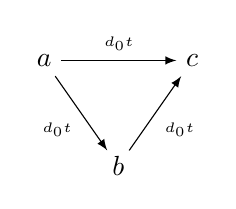
\begin{tikzpicture}%[x=.5cm]
			\node at (160:1) (a) {$a$};
			\node[inner sep=2pt] at (-90:1) (b) {$b$};
			\node at (20:1) (c) {$c$};
			%
			\draw[-latex] (a) -- (b) node[pos=.5,below left,font=\tiny] {$d_0t$};
			\draw[-latex] (b) -- (c) node[pos=.5,below right,font=\tiny] {$d_0t$};
			\draw[-latex] (a) -- (c) node[pos=.5, above, font=\tiny] {$d_0t$};
		\end{tikzpicture}
	\end{center}
\end{hRemark}
\begin{definition}\label{def_insieme_globulare}\index{Insieme!--- globulare}\index{Insieme globulare}
	\index{Insieme!--- globulare}
	Un \emph{insieme globulare} consta di un funtore \(G : \ctGl(n)^\op\fun\ctSet\), dove \(\ctGl(n)\) è la categoria `globo generico' di \ref{ex_globo}.

	Quando la definizione di insieme simpliciale viene data esplicitamente, essa consiste del dato di:
	\begin{itemize}
		\item Una famiglia di insiemi \(G_0,G_1,\dots,G_n\);
		\item Una famiglia di funzioni \(s^n,t^n : G_n\to G_{n-1}\), dette \emph{dominio} e \emph{codominio} \(n\)-dimensionale.
	\end{itemize}
	La funtorialità di \(G\) ora implica che gli elementi di $G_n$ soddisfino a delle condizioni dette \emph{identità globulari}, che discendono da quelle di \ref{}; questa osservazione è espansa in maggior dettaglio in \ref{globi_come_sonfatti}.
\end{definition}
\begin{example}\index{Funtore!--- quoziente di uno pseudoinsieme}
	Sia \((X,\sim)\) un prequoziente come in \ref{ex_cat_pseudoinsiemi}; l'assegnazione del quoziente \(X/_\sim\) definisce un funtore
	\[\dmFun q{\cate{Bish}}{\ctSet}\]
	poiché ogni omomorfismo di pseudoinsiemi \(f : (X,\sim_X)\to (Y,\sim_Y)\) soddisfa esattamente la proprietà necessaria a indurre un'unica funzione \(qf : X/_{\sim_X}\to Y/_{\sim_Y}\), che manda la classe di equivalenza \([x]_X\) nella classe di equivalenza \([fx]_Y\) (si dimostrino per esercizio le identità funtoriali: \(q(\id_{(X,\sim)})=\id_{X/_\sim}\) e \(q(g\cmp f)=qg\cmp qf\)).
\end{example}
\begin{example}\index{Funtore!--- proiezioni da un prodotto}
	\index{Funtore!--- inclusioni in una somma}\index{Categoria!--- somma}
	Le costruzioni in \ref{def_cat_prodotto}, \ref{def_cat_somma} permettono di definire diversi funtori interessanti:
	\begin{itemize}
		\item Dal prodotto \(\ctC\times\ctD\) si possono definire le \emph{proiezioni}
		      % https://q.uiver.app/#q=WzAsMyxbMSwwLCJcXGN0Q1xcdGltZXNcXGN0RCJdLFswLDAsIlxcY3RDIl0sWzIsMCwiXFxjdEQiXSxbMCwyLCJwX1xcY3REIl0sWzAsMSwicF9cXGN0QyIsMl1d
		      \[\begin{tikzcd}
				      \ctC & {\ctC\times\ctD} & \ctD
				      \arrow["{p_\ctC}"', from=1-2, to=1-1]
				      \arrow["{p_\ctD}", from=1-2, to=1-3]
			      \end{tikzcd}\]
		      che agiscono come \(p_\ctC(C,D)=C\) e \(p_\ctD(C,D)=D\) (e similmente sui morfismi \((C\to C', D\to D')\)).
		\item Verso la somma \(\ctC+\ctD\) si possono definire le inclusioni
		      % https://q.uiver.app/#q=WzAsMyxbMSwwLCJcXGN0QytcXGN0RCJdLFswLDAsIlxcY3RDIl0sWzIsMCwiXFxjdEQiXSxbMiwwLCJpX1xcY3REIiwyXSxbMSwwLCJpX1xcY3RDIl1d
		      \[\begin{tikzcd}
				      \ctC & {\ctC+\ctD} & \ctD
				      \arrow["{i_\ctC}", from=1-1, to=1-2]
				      \arrow["{i_\ctD}"', from=1-3, to=1-2]
			      \end{tikzcd}\]
		      che agiscono sugli oggetti immergendo \(\ctC_0,\ctD_0\) nell'unione disgiunta \(\ctC_0+\ctD_0\), e analogamente sui morfismi.
	\end{itemize}
\end{example}
\begin{esercizi}
	\item Descrivere il funtore hom covariante \(\Hom\ctC(C,-)\) e controvariante \(\Hom\ctC(-,C)\) di \ref{ex_hom_funtore} quando: \(\ctC\) ha un solo oggetto, come in \ref{mon_sonocat}; \(\ctC\) è una classe preordinata, come in \ref{ord_sonocat}; \(\ctC = \ctA+\ctB\) è la somma di due categorie fissate; \(\ctC = G\emdash\ctSet\) per un gruppo \(G\) come in \ref{ex_cat_g_insiemi}; \(\ctC = \ctMat\) per un campo \(\bbF\).
	\item Si ricordi la definizione \ref{example_pesati} della categoria \(\cate{wSet}\) degli insiemi pesati. Sia \(\lambda\in[0,\infty]\) un numero reale fissato; definire e studiare le proprietà del funtore `palla di raggio \(\lambda\)'
	\[\dmFun{B_\lambda}{\cate{wSet}}{\ctSet}\]
	che manda \((X,w)\mapsto \{x\in X\mid |x|\le \lambda\}\), con particolare attenzione alle scelte \(\lambda=0,1,\infty\). Il funtore \(B_\lambda\) è pieno? Fedele? Definire funtori \(W_\lambda : \ctSet \fun\cate{wSet}\) nella direzione opposta (sono pieni, fedeli?) tali che se \(\singleton\) denota un qualsiasi singoletto, \(B_\lambda X\) si identifica con l'insieme \(\Hom(W_\lambda\singleton,(X,w))\).
	\item \label{gfdpgubai_1} Mostrare che un funtore \(\ctTerm \fun\ctC\) (un `diagramma di tipo \(\ctTerm = \Delta[0]\)') ammonta precisamente alla scelta di un oggetto di \(\ctC\), e che un diagramma di tipo \(\Delta[1] = \genArrow\) ammonta esattamente alla scelta di una freccia tra due oggetti di \(\ctC\).
	\item \label{gfdpgubai_2} Mostrare che le seguenti condizioni sono equivalenti, nella notazione di \ref{klext_delle_relazioni} per le funzioni \(R^*,R_*\):
	\begin{itemize}
		\item la condizione in \ref{klext_delle_relazioni},
		      \[V\subseteq R^*U\iff U\subseteq R_*V\]
		\item il fatto che per ogni \(U\subseteq B,V\subseteq A\) si abbia
		      \[V\subseteq R^*R_*V\qquad\qquad U\subseteq R_*R^*U\]
	\end{itemize}
	Mostrare che da una qualunque di queste condizioni equivalenti segue che \(R^*,R_*\) sono una coppia di funtori controvarianti, in direzioni opposte:
	\[\begin{tikzcd}
			R^* : (\pow B,\subseteq)^\op \ar[r, shift left] & (\pow A,\subseteq) : R_* \ar[l, shift left]
		\end{tikzcd}\]
	\item \label{gfdpgubai_3} In cosa consiste un funtore
	\[\dmFun F {\act G}\ctSet,\]
	quando \(\act G\) è il gruppoide d'azione di \ref{action_groupoid}? Farsi degli esempi (e dei disegni) quando \(G=C_n\) è il gruppo ciclico con \(n\) elementi, quando \(G=\bbZ\) è il gruppo additivo degli interi, e quando \(G=S_3\) è il gruppo simmetrico delle biiezioni dell'insieme \(\{1,2,3\}\).
	\item \label{gfdpgubai_4} Si costruisca, tramite il differenziale, un funtore simile a quello di \ref{exa_derivata_funtore}, ma sulla categoria \(\cate{Mfd}\) delle varietà e funzioni lisce, che sugli oggetti assegna ad una varietà liscia \(M\) il suo fibrato tangente \(\text{T} M\); tale \(\text{T} M\) è naturalmente equipaggiato con una mappa liscia \(p_M : TM\to M\): il funtore \(\text{T}\) è di tipo \(\cate{Mfd} \to \cate{Mfd}^\to\)? Ovvero, esiste un quadrato commutativo
	\[\xymatrix{
		\text{T} M \ar[r]^{\text{T} f}\ar[d]_{p_M} & \text{T} N \ar[d]^{p_N}\\
		M \ar[r]_f & N
		}\]
	indotto da una mappa liscia \(f : M\to N\) di varietà?
	\item \label{exe_cpt_conn} Definiamo il funtore delle componenti connesse di una categoria
	\[\dmFun{\pi_0^\ctCat}{\ctCat}{\ctSet}\]
	come la composizione del funtore \(\pi_0 : \ctGph \fun\ctSet\) di \ref{ex_fun_cpt_conn} e del funtore \(U : \ctCat \fun\ctGph\) che restituisce il grafo sottostante a una categoria. Diciamo che una categoria \(\ctC\) è connessa quando lo è \(U\ctC\), cioè quando \(\pi_0(U\ctC)\) ha un solo elemento.

	Usando la definizione, calcolare \(\pi_0(A^\delta)\) e \(\pi_0(A^\chi)\) se \(A\) è un insieme (si veda \ref{ex_cat_discreta} e \ref{ex_cat_codiscreta}); calcolare poi
	\begin{itemize}
		\item \(\pi_0(\ctC/X)\) (resp., \(\pi_0(X/\ctC)\)) se \(\ctC\) è una categoria qualsiasi e \(\ctC/X\) l'incubo (resp., la succuba) sopra \(X\);
		\item \(\pi_0(\ctC^\op)\) (come in \ref{def_cat_opp}), è lo stesso di \(\pi_0(\ctC)\)?
		\item \(\pi_0(\ctC\star\ctD)\) (come in \ref{cat_def_giunto}), esiste una coppia di categorie tale che abbia più di un elemento?
		\item \(\pi_0(\act G)\), se \(G\) è un gruppo e \(\act G\) il gruppoide d'azione di \ref{action_groupoid}; cosa significa quando \(\pi_0(\act G)\) non è connesso? (Suggerimento: pensare a \ref{ex_fun_orbite});
		\item Esibire una biiezione, o trovare un controesempio alla sua esistenza, tra \(\pi_0(\ctC\times\ctD)\) e \(\pi_0(\ctC)\times\pi_0(\ctD)\), se \(\ctC\times\ctD\) è il prodotto di categorie di \ref{def_cat_prodotto}; stessa domanda con \(\pi_0(\ctC+\ctD)\) e \(\pi_0(\ctC)+\pi_0(\ctD)\), se \(\ctC+\ctD\) è la somma di categorie di \ref{def_cat_somma}.
	\end{itemize}
\end{esercizi}
